% ****** Start of file apssamp.tex ******
%
%   This file is part of the APS files in the REVTeX 4 distribution.
%   Version 4.0 of REVTeX, August 2001
%
%   Copyright (c) 2001 The American Physical Society.
%
%   See the REVTeX 4 README file for restrictions and more information.
%
% TeX'ing this file requires that you have AMS-LaTeX 2.0 installed
% as well as the rest of the prerequisites for REVTeX 4.0
%
% See the REVTeX 4 README file
% It also requires running BibTeX. The commands are as follows:
%
%  1)  latex apssamp.tex
%  2)  bibtex prb
%  3)  latex apssamp.tex
%  4)  latex apssamp.tex
%
%\documentclass[aps,prb,preprint,groupedaddress,showpacs]{revtex4-1}
\documentclass[aps,prl,preprint,superscriptaddress]{revtex4}
%\documentclass[aps,prl,twocolumn,superscriptaddress]{revtex4}
%\documentclass[aps,prl,twocolumn,superscriptaddress]{revtex4}
%\documentclass[aps,prb,twocolumn,groupedaddress]{revtex4-1}


%\documentclass[twocolumn,showpacs,preprintnumbers,amsmath,amssymb]{revtex4}
%\documentclass[preprint,showpacs,preprintnumbers,amsmath,amssymb]{revtex4}

% Some other (several out of many) possibilities
%\documentclass[preprint,aps]{revtex4}
%\documentclass[preprint,aps,draft]{revtex4}
%\documentclass[prb]{revtex4}% Physical Review B

\usepackage{graphics}
\usepackage{graphicx}% Include figure files
\usepackage{epstopdf}
\usepackage{dcolumn}% Align table columns on decimal point
\usepackage{bm}% bold math
\usepackage{amsmath}
\usepackage{amssymb}
\usepackage{latexsym}
\usepackage{epsfig}
\usepackage{amsbsy}
\usepackage{array}
\usepackage{amssymb}
\usepackage{setspace}
\usepackage{bm}
\usepackage{float}

\newcommand{\ssint}{ - \!\!\!\!\! \int }
\def\sint{\ifmmode{- \!\!\!\!\!\! \int}
    \else{\hbox{$- \!\!\!\! \int \ $}}\fi}


\newcommand{\bsigma}{\boldsymbol{\sigma}}
\newcommand{\bmu}{\boldsymbol{\mu}}
\newcommand{\bvepsilon}{\boldsymbol{\varepsilon}}
\newcommand{\bepsilon}{\boldsymbol{\epsilon}}
\newcommand{\balpha}{\boldsymbol{\alpha}}
\newcommand{\bkappa}{\boldsymbol{\kappa}}
\newcommand{\bchi}{\boldsymbol{\chi}}
\newcommand{\bgamma}{\boldsymbol{\gamma}}
\newcommand{\bpsi}{\boldsymbol{\psi}}
\newcommand{\bnu}{\boldsymbol{\nu}}
\newcommand{\bzero}{\boldsymbol{0}}
\newcommand{\bbeta}{\boldsymbol{\beta}}
\newcommand{\bSigma}{\boldsymbol{\Sigma}}

\newcommand{\va}{\varphi}
\newcommand{\ep}{\epsilon}
\newcommand{\mbf}{{\bf m}}
\newcommand{\pbf}{{\bf p}}
\newcommand{\xbf}{{\bf x}}
\newcommand{\weak}{\rightharpoonup}
\newcommand{\rgoto}{\rightarrow}

\newcommand{\grad}{\mbox{grad}}
\newcommand{\curl}{\mbox{curl}}
\newcommand{\dive}{\mbox{div}}


\newcommand{\tr}{\mbox{tr}}

\newcommand{\ba}{\mathbf{a}}
\newcommand{\bb}{\mathbf{b}}
\newcommand{\bc}{\mathbf{c}}
\newcommand{\bd}{\mathbf{d}}
\newcommand{\be}{\mathbf{e}}
\newcommand{\bsf}{\mathbf{f}}
\newcommand{\bg}{\mathbf{g}}
\newcommand{\bsi}{\mathbf{i}}
\newcommand{\bk}{\mathbf{k}}
\newcommand{\bn}{\mathbf{n}}
\newcommand{\bo}{\mathbf{o}}
\newcommand{\bp}{\mathbf{p}}
\newcommand{\bq}{\mathbf{q}}
\newcommand{\br}{\mathbf{r}}
\newcommand{\bs}{\mathbf{s}}
\newcommand{\bt}{\mathbf{t}}
\newcommand{\bu}{\mathbf{u}}
\newcommand{\bv}{\mathbf{v}}
\newcommand{\bw}{\mathbf{w}}
\newcommand{\bx}{\mathbf{x}}
\newcommand{\by}{\mathbf{y}}
\newcommand{\bz}{\mathbf{z}}

\newcommand{\bca}{\mathbf{A}}
\newcommand{\bcb}{\mathbf{B}}
\newcommand{\bcc}{\mathbf{C}}
\newcommand{\bcd}{\mathbf{D}}
\newcommand{\bce}{\mathbf{E}}
\newcommand{\bcf}{\mathbf{F}}
\newcommand{\bcg}{\mathbf{G}}
\newcommand{\bch}{\mathbf{H}}
\newcommand{\bck}{\mathbf{K}}
\newcommand{\bcj}{\mathbf{J}}
\newcommand{\bci}{\mathbf{I}}
\newcommand{\bcl}{\mathbf{L}}
\newcommand{\bcm}{\mathbf{M}}
\newcommand{\bcn}{\mathbf{N}}
\newcommand{\bco}{\mathbf{O}}
\newcommand{\bcp}{\mathbf{P}}
\newcommand{\bcq}{\mathbf{Q}}
\newcommand{\bcr}{\mathbf{R}}
\newcommand{\bcs}{\mathbf{S}}
\newcommand{\bct}{\mathbf{T}}
\newcommand{\bcu}{\mathbf{U}}
\newcommand{\bcv}{\mathbf{V}}
\newcommand{\bcw}{\mathbf{W}}
\newcommand{\bcx}{\mathbf{X}}
\newcommand{\bcz}{\mathbf{Z}}
\newcommand{\bcy}{\mathbf{Y}}

%\nofiles

\begin{document}
	
	
	\title{Random Walk, Diffusion and Cluster Growth}% Force line breaks with \\
	
	\author{Xinyu Wu, Peifan Liu, Connor Hann and Xiaomeng Jia}
	\affiliation{Physics Department, Duke University}
	
	
	\date{\today}
	
	\begin{abstract}
		In this article,  
	\end{abstract}
	
	\maketitle
	
	
	
	\section{1. 2D Random Walk} 
	
	
	A random walk is a mathematical formalization of a path that consists of a succession of random steps. For one dimensional case, a random walker can move one step in $\pm x$ directions with equal probability at each time step. If we make consider the statistical properties of  an ensemble of random walkers, the expected value of the position $ <x> $ is zero, since the expectation of each step is zero. However, the root-mean-squared distance(RMS) after n steps is:
	
	\begin{equation}
	\sqrt{<x_n^2>} = \sqrt{\sum\limits_{i=1}^{n}\sum\limits_{j=1}^{n}<\Delta x_i\Delta x_j>} = \sqrt{n}\Delta x
	\end{equation} 
	Here $\Delta x$ is the step unit corresponding to a time unit $\Delta t$ and a constant velocity $v$:
	\begin{equation}
	\Delta x = v\cdot \Delta t
	\end{equation} 
	Combined with
	\begin{equation}
	n = \frac{t}{\Delta t}
	\end{equation}
	We can show that the motion is diffusive:
	\begin{equation}
	<x^2(t)> = 2Dt
	\end{equation}
	where $D = v\cdot\Delta x/2 = (\Delta x)^2/(2\Delta t)$ is the diffusion constant.
	
	If we generalize the deduction to the 2D case, where the random walkers can move one step in four diections ($\pm x, \pm y$) with equal probability, we can find that the motion is again diffusive, by evaluating the mean square distance:
	
	\begin{equation}
	<r^2(t)> = 2Dt
	\end{equation}
	Where $D = (\Delta x)^2/(4\Delta t)$.
	
	This argument can be verified numerically using Python. We write a program to simulate a random walker in 2 dimensions, taking steps
	of unit length in $\pm x$ or $\pm y$ direction on a discrete square lattice. For up to $n = 100$, by averaging over $10^4$ different walks for each $n > 3$, the expected value of the position $ <x> $ is zero at all time, and the mean square value  $ <x^2> $ has a linear relation with $n$(remember $n =t/\Delta t$ is proportional to $t$), as can be seen in Fig.1. A typical 2D random walking pattern is show in Fig.2. Since we choose $\Delta t = \Delta x = 1$ here, the diffusion constant is determined using the slope of $<r^2(t)>$ and $n$(see Fig.3):$D = 1/4$. 
	
		\begin{figure}[H]
			\centering
			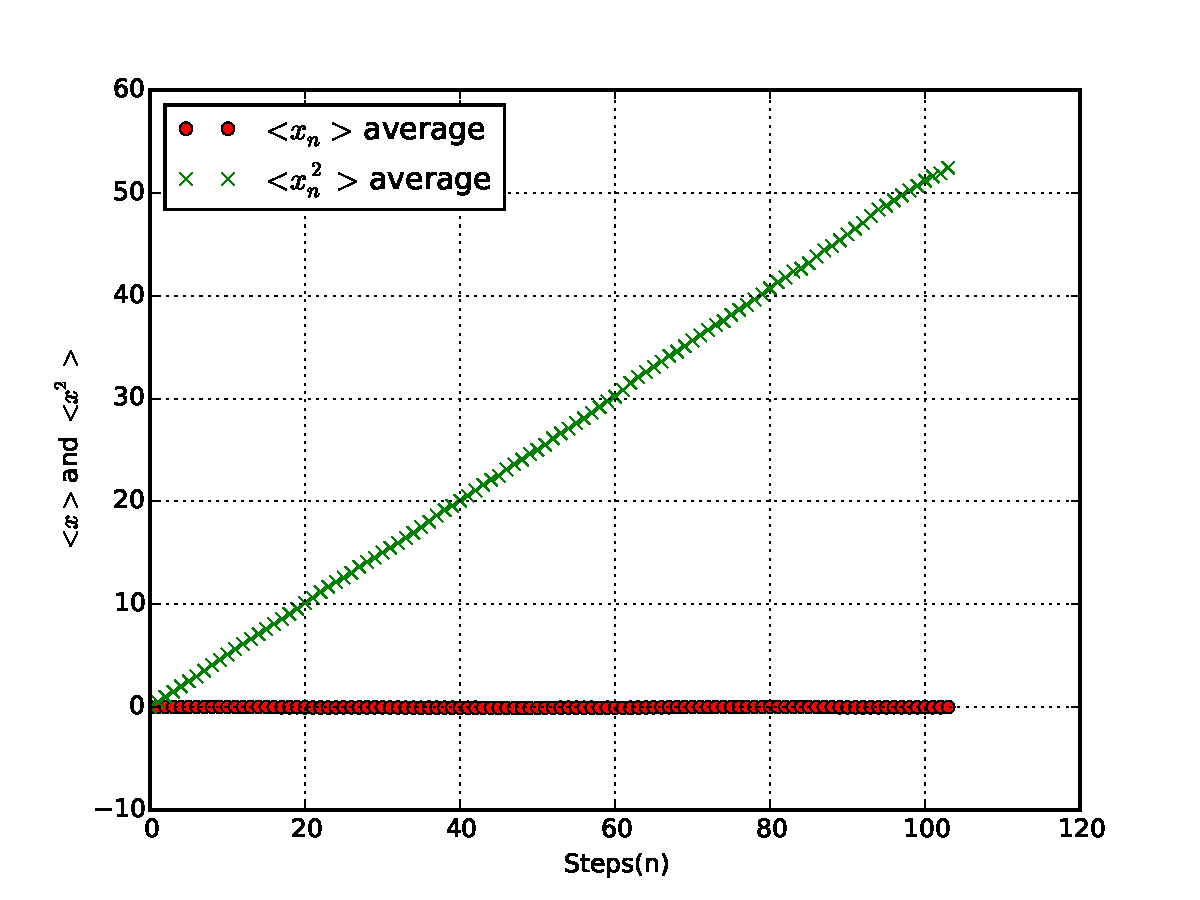
\includegraphics[width=1.0\textwidth]{rwxn.pdf}
			\caption{$ <x(t)> $ and  $ <x^2(t)> $ in 1D random walking, averaging over a 10000 random walker ensemble.}
		\end{figure}
			\begin{figure}[H]
				\centering
				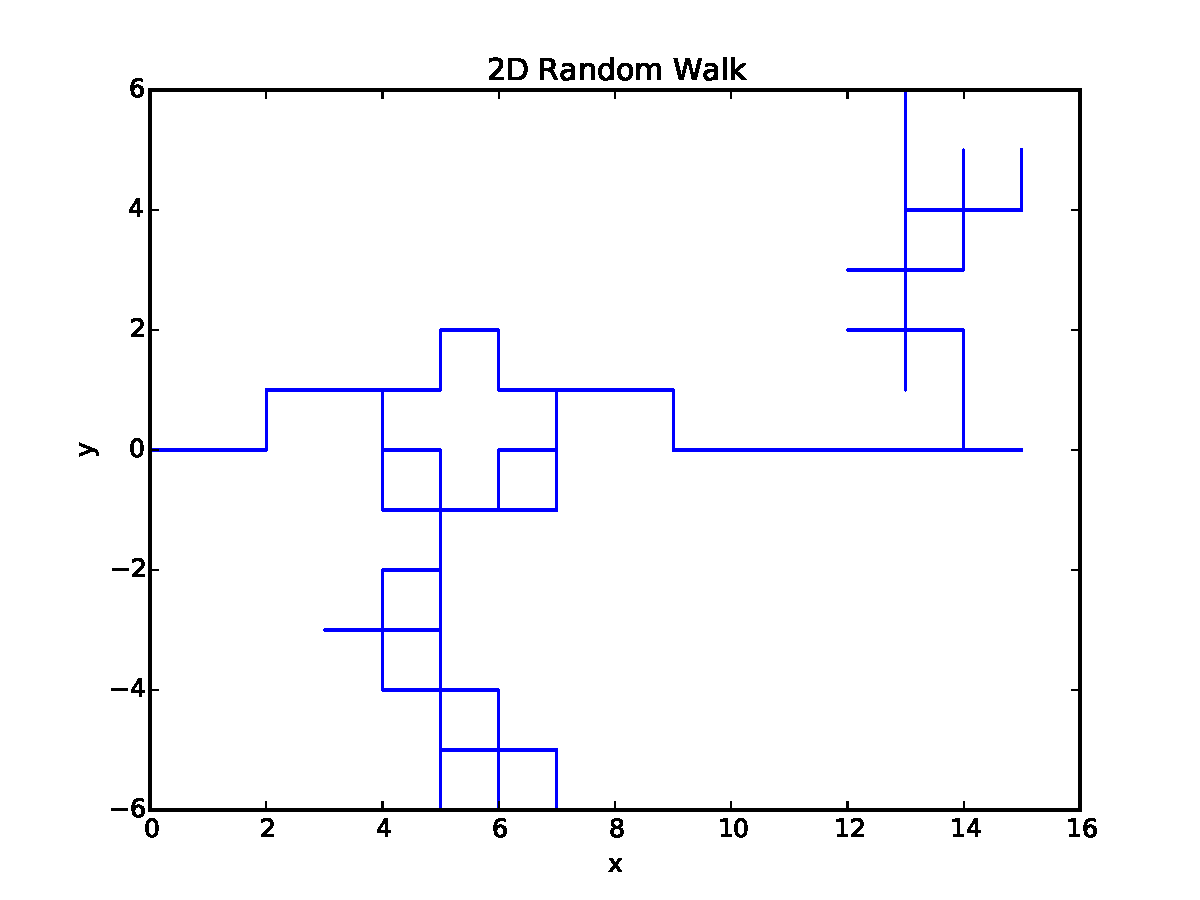
\includegraphics[width=1.0\textwidth]{rwxn3.pdf}
				\caption{A tipical 2D random walking pattern, starting from (0,0).}
			\end{figure}
		\begin{figure}[H]
			\centering
			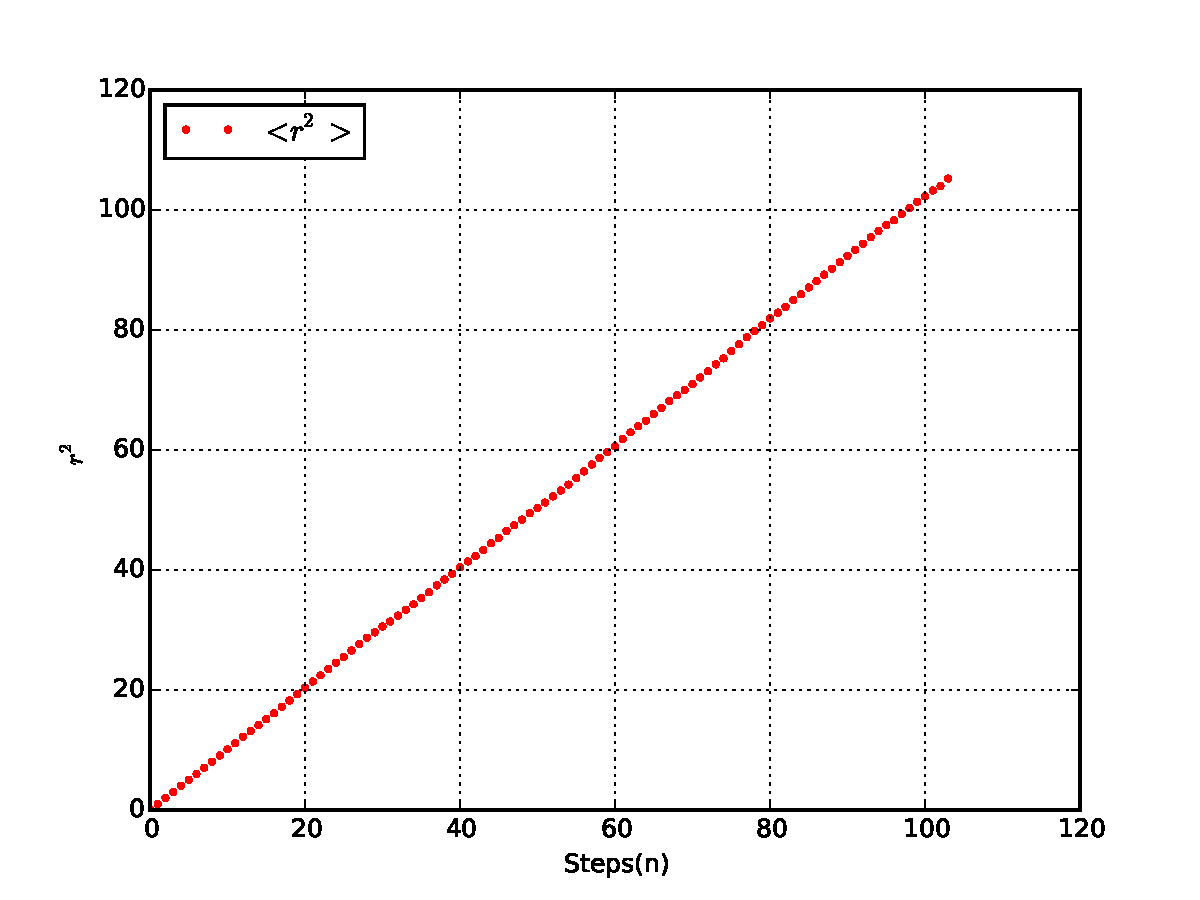
\includegraphics[width=1.0\textwidth]{rwxn2.pdf}
			\caption{$<r^2(t)>$ in 2D random walking, averaging over a 10000 random walker ensemble.}
		\end{figure}

	
	\section{2. Diffusion Equation}
	In this problem we aim to simulate the diffusion of one substance diffusion in another(sugar in water for instance). Diffusion will start from a box profile with a peak at origin and 10 grid around and diffuse in 1 dimension. We will found out the diffusion will approximate Gaussian distribution at later times and fit will be preformed to verify that $\sigma=\sqrt{2Dt}$ for several snapshot t.

\begin{enumerate}
\item First of all we will show analytically that the spatial expectation $\langle x(t)^2\rangle$ of the 1D normal distribution 
\begin{equation}
\rho_{(x,t)}=\frac{1}{\sqrt{2\pi}\sigma{(t)}}\exp(-\frac{x^2}{2\sigma{(t)}^2})
\end{equation}
is just $\sigma(t)^2$.

The spatial expectation
\begin{equation}
\begin{split}
\langle x(t)^2\rangle&=\int_{-\infty}^{\infty}\frac{1}{\sqrt{2\pi}\sigma(t)}x^2\exp(-\frac{x^2}{2\sigma(t)^2})dx\\
&=\frac{1}{\sqrt{2\pi}\sigma(t)}\int_{-\infty}^{\infty}x^2\exp(-\frac{x^2}{2\sigma(t)^2})dx\\
&=\frac{1}{\sqrt{2\pi}\sigma(t)}\times \sqrt{2\pi}\sigma(t)^3\\
&=\sigma(t)^2.
\end{split}
\end{equation}

So $\langle x(t)^2\rangle=\sigma(t)^2$.
\item We know the diffusion equation
\begin{equation}
\frac{\partial\rho}{\partial t}=D\nabla^2\rho
\end{equation}
If we discretize time and position to $t=k\Delta t, x=i\Delta x$, we can get the recursion equation with time, 
\begin{equation}
\rho_{i,k+1}=\rho_{i,k}+D\frac{\Delta t}{\Delta x^2}(\rho_{i+1,k}+\rho_{i-1,k}-2\rho_{i,k})
\end{equation}
here we used $\Delta t=0.002s, \Delta x=0.1m, D=2$. The relation $\Delta t=\frac{\Delta x^2}{2D}$ is satisfied to guarantee convergence.

Then, with the initial distribution given, all future state can be solved. We here will solve the equation for 150s and take snapshot at 30s, 60s, 90s, 120s and 150s. Gaussian fit is applied to these snapshot to verify $\sigma=\sqrt{2Dt}$. Plots for the 5 snapshots and fitted Gaussian are shown in Fig. \ref{fig:diffusion1}.
\begin{figure}
\centering
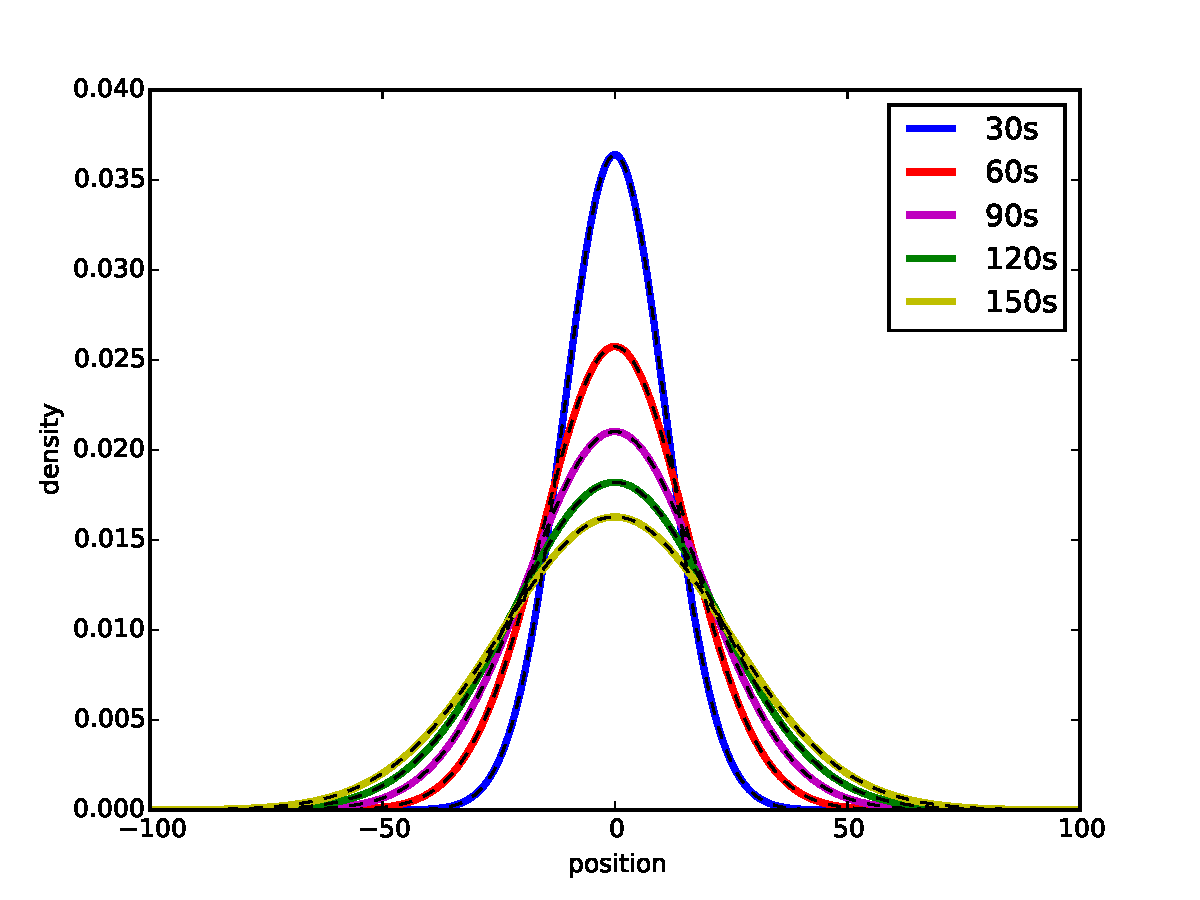
\includegraphics[scale=0.85]{diffusion.pdf}
\caption{Snapshots at 30s, 60s, 90s, 120s, 150s and comparison with fitted curve}
\label{fig:diffusion1}
\end{figure}

As for the Gaussian fit, we used the function curve\_fit from scipy.optimize. We first define the Gaussian function with input of $x, \mu, \sigma$ and call it in the function \_fit to get the optimized $\sigma$ the comparison of $\sigma$ with $\sqrt{2Dt}$ are shown in Fig. \ref{fig:diffusion2}.
\begin{figure}
\centering
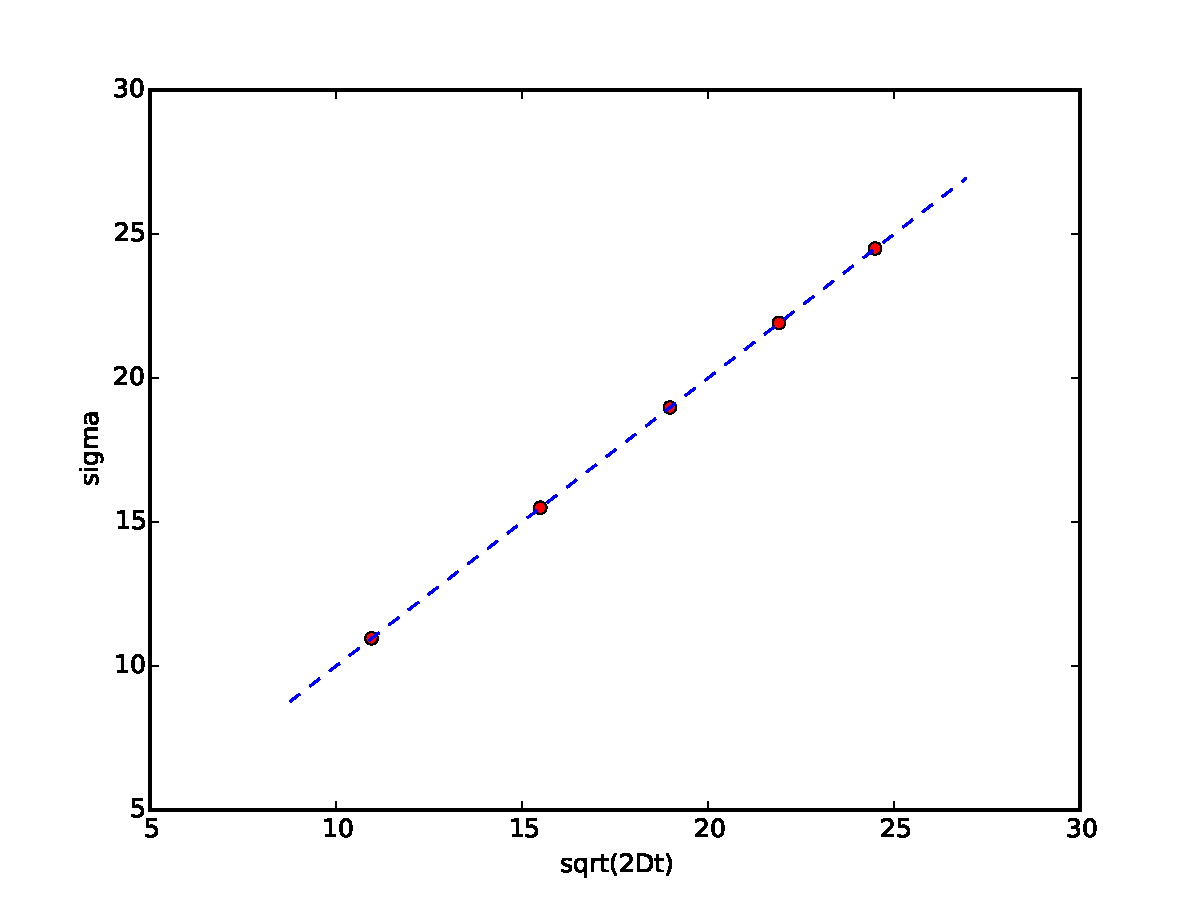
\includegraphics[scale=0.75]{sigma.pdf}
\caption{Comparison of $\sigma$ and $\sqrt{2Dt}$, the blue dashed line is $y=x$.}\label{fig:diffusion2}
\end{figure}

\textbf{\textit{Discussion}}

In this problem, we used the diffusion equation to simulate the diffusion of a initial distribution of a peak(spread out a few grid) and we find that the distribution tend to approximate Gaussian distribution. We also find that the spatial spread expectation $\langle x(t)^2\rangle=2Dt$ increase linearly with time.
\end{enumerate}

	\section{3. Cluster Growth with the DLA model}

Diffusion-limited aggregation (DLA) is the process whereby particles undergoing a random walk due to Brownian motion cluster together to form aggregates of such particles. This theory, proposed by T.A. Witten Jr. and L.M. Sander in 1981, is applicable to aggregation in any system where diffusion is the primary means of transport in the system. DLA can be observed in many systems such as electrodeposition, Hele-Shaw flow, mineral deposits, and dielectric breakdown.
\begin{enumerate}
\item
		\begin{figure}[H]
			\centering
			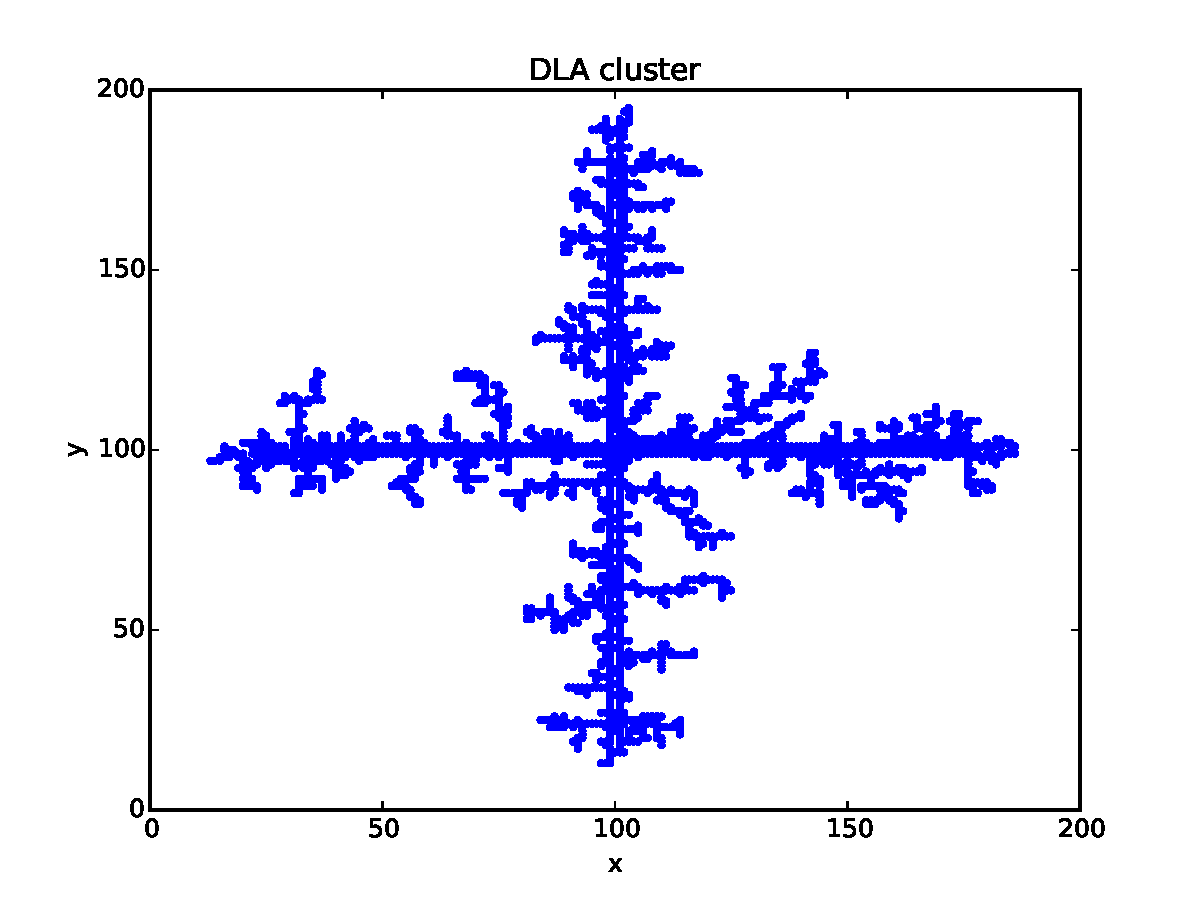
\includegraphics[width=1.0\textwidth]{dla.pdf}
			\caption{DLA Cluster.}
		\end{figure}
\item
\item
		\begin{figure}[H]
			\centering
			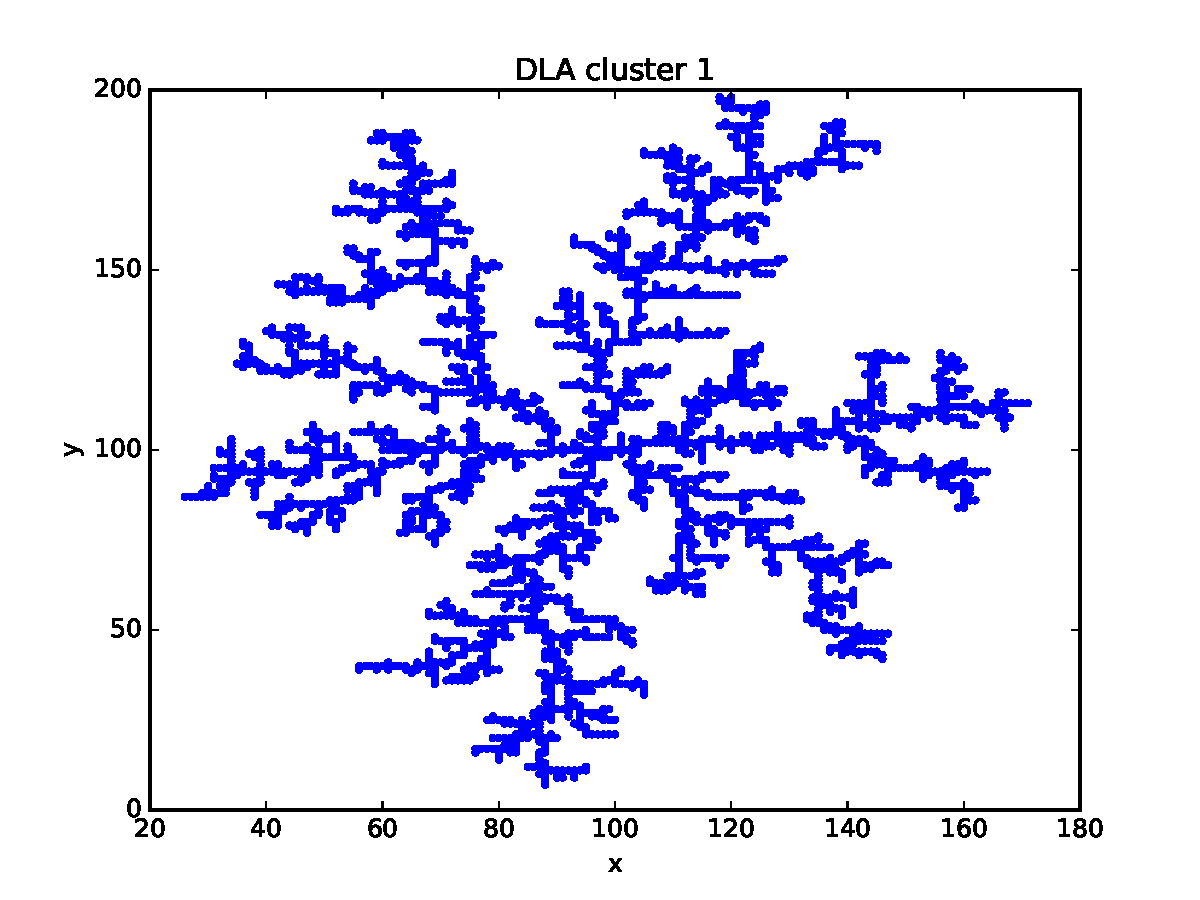
\includegraphics[width=1.0\textwidth]{dla_0.pdf}
			\caption{DLA cluster 1.}
		\end{figure}
				\begin{figure}[H]
			\centering
			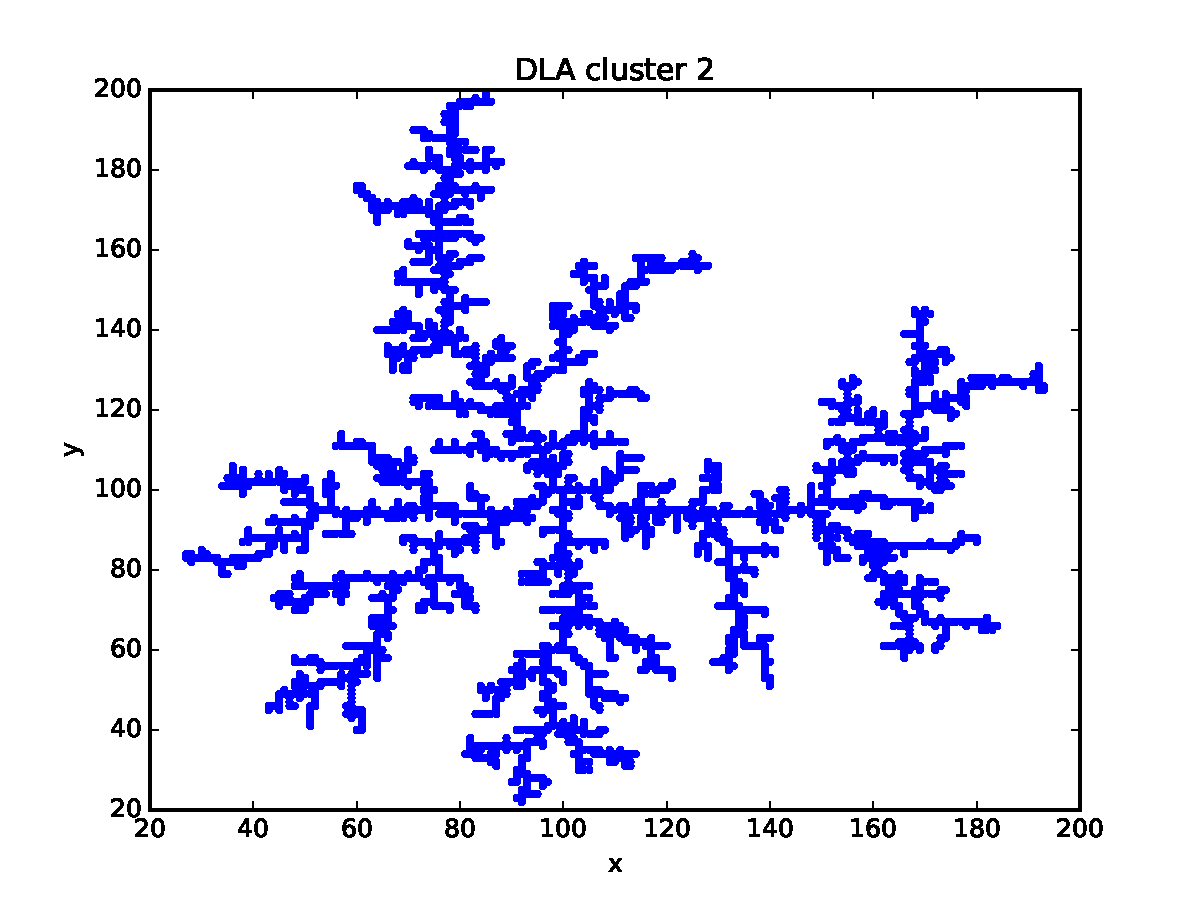
\includegraphics[width=1.0\textwidth]{dla_1.pdf}
			\caption{DLA cluster 2.}
		\end{figure}
				\begin{figure}[H]
			\centering
			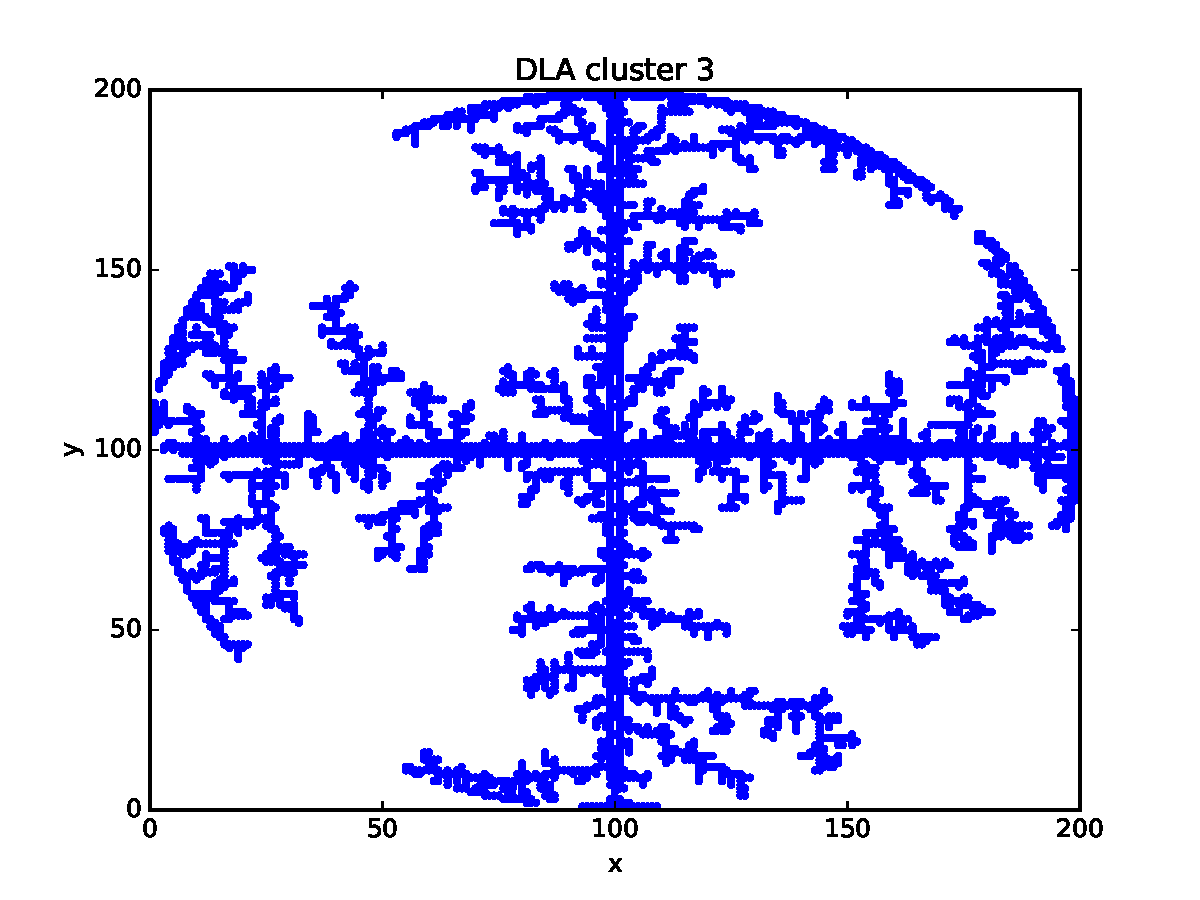
\includegraphics[width=1.0\textwidth]{dla_2.pdf}
			\caption{DLA cluster 3.}
		\end{figure}
				\begin{figure}[H]
			\centering
			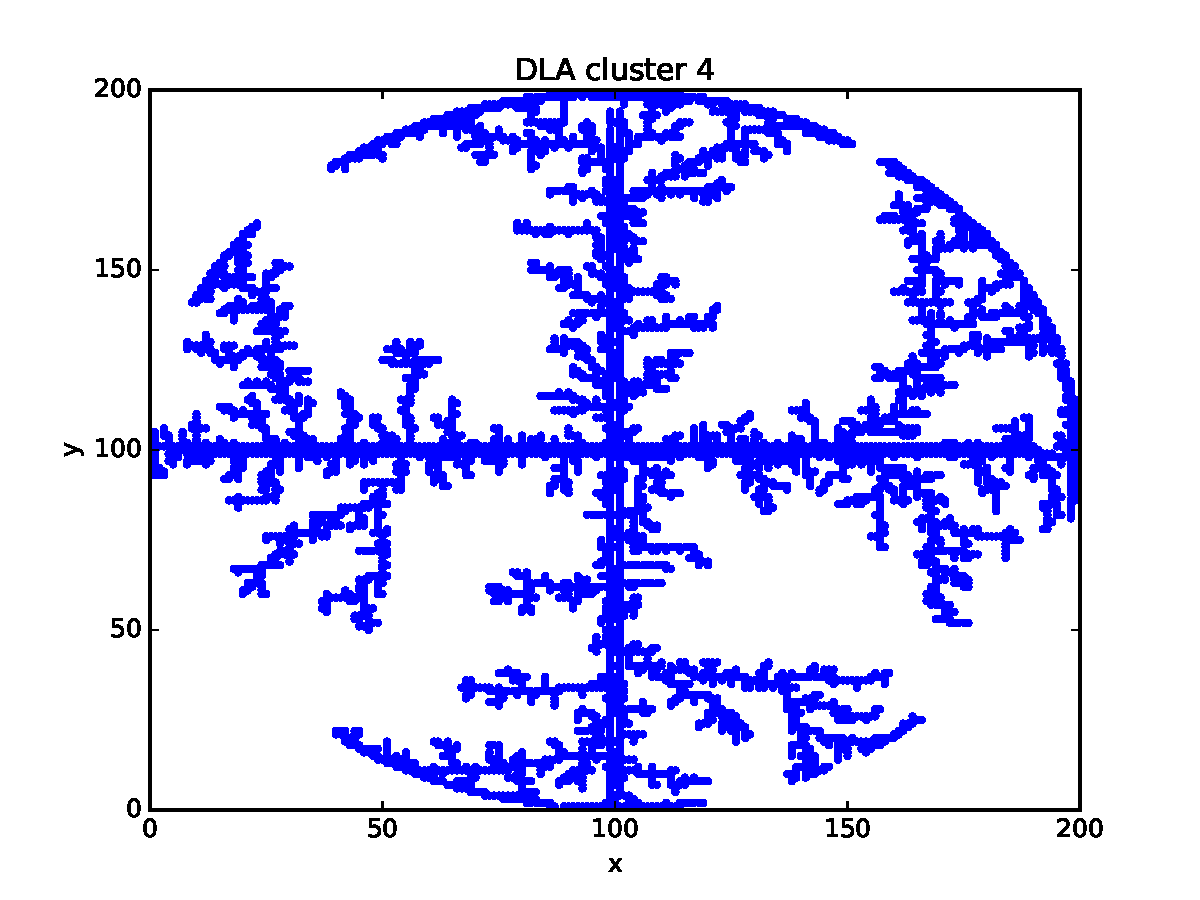
\includegraphics[width=1.0\textwidth]{dla_3.pdf}
			\caption{DLA cluster 4.}
		\end{figure}
\end{enumerate}

	
\end{document}
	
	%
	% ****** End of file apssamp.tex ******
